% Generated by Sphinx.
\def\sphinxdocclass{report}
\documentclass[letterpaper,10pt,english]{sphinxmanual}
\usepackage[utf8]{inputenc}
\DeclareUnicodeCharacter{00A0}{\nobreakspace}
\usepackage{cmap}
\usepackage[T1]{fontenc}
\usepackage{babel}
\usepackage{times}
\usepackage[Bjarne]{fncychap}
\usepackage{longtable}
\usepackage{sphinx}
\usepackage{multirow}

\addto\captionsenglish{\renewcommand{\figurename}{Fig. }}
\addto\captionsenglish{\renewcommand{\tablename}{Table }}
\floatname{literal-block}{Listing }



\title{Practical 13: AdK Tutorial Documentation}
\date{June 10, 2015}
\release{1.0}
\author{Oliver Beckstein}
\newcommand{\sphinxlogo}{}
\renewcommand{\releasename}{Release}
\makeindex

\makeatletter
\def\PYG@reset{\let\PYG@it=\relax \let\PYG@bf=\relax%
    \let\PYG@ul=\relax \let\PYG@tc=\relax%
    \let\PYG@bc=\relax \let\PYG@ff=\relax}
\def\PYG@tok#1{\csname PYG@tok@#1\endcsname}
\def\PYG@toks#1+{\ifx\relax#1\empty\else%
    \PYG@tok{#1}\expandafter\PYG@toks\fi}
\def\PYG@do#1{\PYG@bc{\PYG@tc{\PYG@ul{%
    \PYG@it{\PYG@bf{\PYG@ff{#1}}}}}}}
\def\PYG#1#2{\PYG@reset\PYG@toks#1+\relax+\PYG@do{#2}}

\expandafter\def\csname PYG@tok@gd\endcsname{\def\PYG@tc##1{\textcolor[rgb]{0.63,0.00,0.00}{##1}}}
\expandafter\def\csname PYG@tok@gu\endcsname{\let\PYG@bf=\textbf\def\PYG@tc##1{\textcolor[rgb]{0.50,0.00,0.50}{##1}}}
\expandafter\def\csname PYG@tok@gt\endcsname{\def\PYG@tc##1{\textcolor[rgb]{0.00,0.27,0.87}{##1}}}
\expandafter\def\csname PYG@tok@gs\endcsname{\let\PYG@bf=\textbf}
\expandafter\def\csname PYG@tok@gr\endcsname{\def\PYG@tc##1{\textcolor[rgb]{1.00,0.00,0.00}{##1}}}
\expandafter\def\csname PYG@tok@cm\endcsname{\let\PYG@it=\textit\def\PYG@tc##1{\textcolor[rgb]{0.25,0.50,0.56}{##1}}}
\expandafter\def\csname PYG@tok@vg\endcsname{\def\PYG@tc##1{\textcolor[rgb]{0.73,0.38,0.84}{##1}}}
\expandafter\def\csname PYG@tok@m\endcsname{\def\PYG@tc##1{\textcolor[rgb]{0.13,0.50,0.31}{##1}}}
\expandafter\def\csname PYG@tok@mh\endcsname{\def\PYG@tc##1{\textcolor[rgb]{0.13,0.50,0.31}{##1}}}
\expandafter\def\csname PYG@tok@cs\endcsname{\def\PYG@tc##1{\textcolor[rgb]{0.25,0.50,0.56}{##1}}\def\PYG@bc##1{\setlength{\fboxsep}{0pt}\colorbox[rgb]{1.00,0.94,0.94}{\strut ##1}}}
\expandafter\def\csname PYG@tok@ge\endcsname{\let\PYG@it=\textit}
\expandafter\def\csname PYG@tok@vc\endcsname{\def\PYG@tc##1{\textcolor[rgb]{0.73,0.38,0.84}{##1}}}
\expandafter\def\csname PYG@tok@il\endcsname{\def\PYG@tc##1{\textcolor[rgb]{0.13,0.50,0.31}{##1}}}
\expandafter\def\csname PYG@tok@go\endcsname{\def\PYG@tc##1{\textcolor[rgb]{0.20,0.20,0.20}{##1}}}
\expandafter\def\csname PYG@tok@cp\endcsname{\def\PYG@tc##1{\textcolor[rgb]{0.00,0.44,0.13}{##1}}}
\expandafter\def\csname PYG@tok@gi\endcsname{\def\PYG@tc##1{\textcolor[rgb]{0.00,0.63,0.00}{##1}}}
\expandafter\def\csname PYG@tok@gh\endcsname{\let\PYG@bf=\textbf\def\PYG@tc##1{\textcolor[rgb]{0.00,0.00,0.50}{##1}}}
\expandafter\def\csname PYG@tok@ni\endcsname{\let\PYG@bf=\textbf\def\PYG@tc##1{\textcolor[rgb]{0.84,0.33,0.22}{##1}}}
\expandafter\def\csname PYG@tok@nl\endcsname{\let\PYG@bf=\textbf\def\PYG@tc##1{\textcolor[rgb]{0.00,0.13,0.44}{##1}}}
\expandafter\def\csname PYG@tok@nn\endcsname{\let\PYG@bf=\textbf\def\PYG@tc##1{\textcolor[rgb]{0.05,0.52,0.71}{##1}}}
\expandafter\def\csname PYG@tok@no\endcsname{\def\PYG@tc##1{\textcolor[rgb]{0.38,0.68,0.84}{##1}}}
\expandafter\def\csname PYG@tok@na\endcsname{\def\PYG@tc##1{\textcolor[rgb]{0.25,0.44,0.63}{##1}}}
\expandafter\def\csname PYG@tok@nb\endcsname{\def\PYG@tc##1{\textcolor[rgb]{0.00,0.44,0.13}{##1}}}
\expandafter\def\csname PYG@tok@nc\endcsname{\let\PYG@bf=\textbf\def\PYG@tc##1{\textcolor[rgb]{0.05,0.52,0.71}{##1}}}
\expandafter\def\csname PYG@tok@nd\endcsname{\let\PYG@bf=\textbf\def\PYG@tc##1{\textcolor[rgb]{0.33,0.33,0.33}{##1}}}
\expandafter\def\csname PYG@tok@ne\endcsname{\def\PYG@tc##1{\textcolor[rgb]{0.00,0.44,0.13}{##1}}}
\expandafter\def\csname PYG@tok@nf\endcsname{\def\PYG@tc##1{\textcolor[rgb]{0.02,0.16,0.49}{##1}}}
\expandafter\def\csname PYG@tok@si\endcsname{\let\PYG@it=\textit\def\PYG@tc##1{\textcolor[rgb]{0.44,0.63,0.82}{##1}}}
\expandafter\def\csname PYG@tok@s2\endcsname{\def\PYG@tc##1{\textcolor[rgb]{0.25,0.44,0.63}{##1}}}
\expandafter\def\csname PYG@tok@vi\endcsname{\def\PYG@tc##1{\textcolor[rgb]{0.73,0.38,0.84}{##1}}}
\expandafter\def\csname PYG@tok@nt\endcsname{\let\PYG@bf=\textbf\def\PYG@tc##1{\textcolor[rgb]{0.02,0.16,0.45}{##1}}}
\expandafter\def\csname PYG@tok@nv\endcsname{\def\PYG@tc##1{\textcolor[rgb]{0.73,0.38,0.84}{##1}}}
\expandafter\def\csname PYG@tok@s1\endcsname{\def\PYG@tc##1{\textcolor[rgb]{0.25,0.44,0.63}{##1}}}
\expandafter\def\csname PYG@tok@gp\endcsname{\let\PYG@bf=\textbf\def\PYG@tc##1{\textcolor[rgb]{0.78,0.36,0.04}{##1}}}
\expandafter\def\csname PYG@tok@sh\endcsname{\def\PYG@tc##1{\textcolor[rgb]{0.25,0.44,0.63}{##1}}}
\expandafter\def\csname PYG@tok@ow\endcsname{\let\PYG@bf=\textbf\def\PYG@tc##1{\textcolor[rgb]{0.00,0.44,0.13}{##1}}}
\expandafter\def\csname PYG@tok@sx\endcsname{\def\PYG@tc##1{\textcolor[rgb]{0.78,0.36,0.04}{##1}}}
\expandafter\def\csname PYG@tok@bp\endcsname{\def\PYG@tc##1{\textcolor[rgb]{0.00,0.44,0.13}{##1}}}
\expandafter\def\csname PYG@tok@c1\endcsname{\let\PYG@it=\textit\def\PYG@tc##1{\textcolor[rgb]{0.25,0.50,0.56}{##1}}}
\expandafter\def\csname PYG@tok@kc\endcsname{\let\PYG@bf=\textbf\def\PYG@tc##1{\textcolor[rgb]{0.00,0.44,0.13}{##1}}}
\expandafter\def\csname PYG@tok@c\endcsname{\let\PYG@it=\textit\def\PYG@tc##1{\textcolor[rgb]{0.25,0.50,0.56}{##1}}}
\expandafter\def\csname PYG@tok@mf\endcsname{\def\PYG@tc##1{\textcolor[rgb]{0.13,0.50,0.31}{##1}}}
\expandafter\def\csname PYG@tok@err\endcsname{\def\PYG@bc##1{\setlength{\fboxsep}{0pt}\fcolorbox[rgb]{1.00,0.00,0.00}{1,1,1}{\strut ##1}}}
\expandafter\def\csname PYG@tok@mb\endcsname{\def\PYG@tc##1{\textcolor[rgb]{0.13,0.50,0.31}{##1}}}
\expandafter\def\csname PYG@tok@ss\endcsname{\def\PYG@tc##1{\textcolor[rgb]{0.32,0.47,0.09}{##1}}}
\expandafter\def\csname PYG@tok@sr\endcsname{\def\PYG@tc##1{\textcolor[rgb]{0.14,0.33,0.53}{##1}}}
\expandafter\def\csname PYG@tok@mo\endcsname{\def\PYG@tc##1{\textcolor[rgb]{0.13,0.50,0.31}{##1}}}
\expandafter\def\csname PYG@tok@kd\endcsname{\let\PYG@bf=\textbf\def\PYG@tc##1{\textcolor[rgb]{0.00,0.44,0.13}{##1}}}
\expandafter\def\csname PYG@tok@mi\endcsname{\def\PYG@tc##1{\textcolor[rgb]{0.13,0.50,0.31}{##1}}}
\expandafter\def\csname PYG@tok@kn\endcsname{\let\PYG@bf=\textbf\def\PYG@tc##1{\textcolor[rgb]{0.00,0.44,0.13}{##1}}}
\expandafter\def\csname PYG@tok@o\endcsname{\def\PYG@tc##1{\textcolor[rgb]{0.40,0.40,0.40}{##1}}}
\expandafter\def\csname PYG@tok@kr\endcsname{\let\PYG@bf=\textbf\def\PYG@tc##1{\textcolor[rgb]{0.00,0.44,0.13}{##1}}}
\expandafter\def\csname PYG@tok@s\endcsname{\def\PYG@tc##1{\textcolor[rgb]{0.25,0.44,0.63}{##1}}}
\expandafter\def\csname PYG@tok@kp\endcsname{\def\PYG@tc##1{\textcolor[rgb]{0.00,0.44,0.13}{##1}}}
\expandafter\def\csname PYG@tok@w\endcsname{\def\PYG@tc##1{\textcolor[rgb]{0.73,0.73,0.73}{##1}}}
\expandafter\def\csname PYG@tok@kt\endcsname{\def\PYG@tc##1{\textcolor[rgb]{0.56,0.13,0.00}{##1}}}
\expandafter\def\csname PYG@tok@sc\endcsname{\def\PYG@tc##1{\textcolor[rgb]{0.25,0.44,0.63}{##1}}}
\expandafter\def\csname PYG@tok@sb\endcsname{\def\PYG@tc##1{\textcolor[rgb]{0.25,0.44,0.63}{##1}}}
\expandafter\def\csname PYG@tok@k\endcsname{\let\PYG@bf=\textbf\def\PYG@tc##1{\textcolor[rgb]{0.00,0.44,0.13}{##1}}}
\expandafter\def\csname PYG@tok@se\endcsname{\let\PYG@bf=\textbf\def\PYG@tc##1{\textcolor[rgb]{0.25,0.44,0.63}{##1}}}
\expandafter\def\csname PYG@tok@sd\endcsname{\let\PYG@it=\textit\def\PYG@tc##1{\textcolor[rgb]{0.25,0.44,0.63}{##1}}}

\def\PYGZbs{\char`\\}
\def\PYGZus{\char`\_}
\def\PYGZob{\char`\{}
\def\PYGZcb{\char`\}}
\def\PYGZca{\char`\^}
\def\PYGZam{\char`\&}
\def\PYGZlt{\char`\<}
\def\PYGZgt{\char`\>}
\def\PYGZsh{\char`\#}
\def\PYGZpc{\char`\%}
\def\PYGZdl{\char`\$}
\def\PYGZhy{\char`\-}
\def\PYGZsq{\char`\'}
\def\PYGZdq{\char`\"}
\def\PYGZti{\char`\~}
% for compatibility with earlier versions
\def\PYGZat{@}
\def\PYGZlb{[}
\def\PYGZrb{]}
\makeatother

\renewcommand\PYGZsq{\textquotesingle}

\begin{document}

\maketitle
\tableofcontents
\phantomsection\label{index::doc}


{\hfill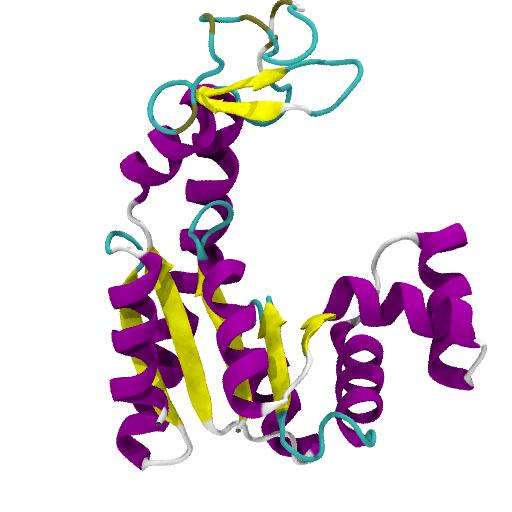
\includegraphics[width=0.300\linewidth]{adk_secondary.jpg}}

\textbf{Objective}: Perform aa MD simulation of the the enzyme adenylate kinase
(AdK) in its open conformation without a ligand bound. Simulate it in
a realistic environment (100 mM NaCl solution at \(T = 300\) K and
\(P = 1\) bar) and analyze its structural properties.

This tutorial progresses through the individual steps needed to set up
and run an equilibrium MD simulation of AdK using Gromacs.
\paragraph{Workflow summary}


\chapter{Directory organization}
\label{directory_organization:directory-organization}\label{directory_organization::doc}\label{directory_organization:tutorial-simulating-adk-with-gromacs}
The workflow for setting up, running, and analysing a simulation
consists of multiple and rather different steps. It is useful to
perform these different steps in separate directories in order to
avoid overwriting files or using wrong files.

\textbf{Directory layout}
\begin{quote}

For this tutorial the suggested directory layout is the following:

\begin{Verbatim}[commandchars=\\\{\}]
coord/
top/
solvation/
emin/
posres/
MD/
analysis/
\end{Verbatim}

You will work through these directories in sequence.
\end{quote}
\paragraph{Short description of the directories}
\begin{description}
\item[{\code{coord}}] \leavevmode
original PDB (structural) files

\item[{\code{top}}] \leavevmode
generating topology files (\code{.top}, \code{.itp})

\item[{\code{solvation}}] \leavevmode
adding solvent and ions to the system

\item[{\code{emin}}] \leavevmode
performing energy minimization

\item[{\code{posres}}] \leavevmode
short MD simulation with position restraints on the heavy protein
atoms, to allow the solvent to equilibrate around the protein
without disturbing the protein structure

\item[{\code{MD}}] \leavevmode
MD simulation (typically, you will transfer the \code{md.tpr} file to a
supercomputer, run the simulation there, then copy the the output
back to this trajctory)

\item[{\code{analysis}}] \leavevmode
post-processing a production trajectory to facilitate easy visualization
(i.e., using VMD); analysis of the simulations can be placed in
(sub)directories under analysis, e.g.

\begin{Verbatim}[commandchars=\\\{\}]
\PYG{n}{analysis}\PYG{o}{/}\PYG{n}{RMSD}
\PYG{n}{analysis}\PYG{o}{/}\PYG{n}{RMSF}
\PYG{o}{.}\PYG{o}{.}\PYG{o}{.}
\end{Verbatim}

The subdirectories depend on the specific analysis tasks that you
want to carry out. The above directory layout is only a suggestion
but in practice some sort of ordered directory hierarchy has proven
very useful.

\end{description}

\begin{notice}{note}{Note:}
The command snippets in this tutorial assume the above directory layout.
The workflow is such that each step is carried out
\emph{inside the appropriate directory} and \emph{relative} paths are used to
access files from previous steps. It should be clear from the context
in which directory the commands are to be executed. If you get a
\code{File input/output error} from \textbf{\texttt{grompp}} (or any of the
other commands) then check that you are able to see the file by just
doing a \code{ls ../path/to/file} from where you are in the file system.
If you can't see the file then check (1) that you are in the correct
directory, (2) that you have created the file in a previous step.
\end{notice}


\chapter{Setup of the solvated protein system}
\label{system_setup:setup}\label{system_setup::doc}\label{system_setup:setup-of-the-solvated-protein-system}\label{system_setup:atom-record-of-a-pdb-file}

\section{Directory setup}
\label{system_setup:directory-setup}\begin{itemize}
\item {} 
Create directories that reflects our workflow:

\begin{Verbatim}[commandchars=\\\{\}]
mkdir top solvation emin posres MD analysis
\end{Verbatim}

\item {} 
Optional: get \href{http://www.rcsb.org/pdb/explore.do?structureId=4ake}{4AKE} and only keep chain A:

\begin{notice}{note}{Note:}
The starting structure \code{coord/4ake\_a.pdb} has been
provided as part of the tutorial package so the
instructions here are simply telling you what you would
need to do if the file hadn't been provided.
\end{notice}
\begin{itemize}
\item {} 
Download from the protein databank through the web interface (pdb:
\href{http://www.rcsb.org/pdb/explore.do?structureId=4ake}{4AKE})

\item {} 
Modify the structure; in simple cases such as the one here, you
can just open the PDB file in a text editor and remove all the
lines that are not needed. In more difficult cases you might have
to use molecular modeling software.
\begin{itemize}
\item {} 
Remove all comment lines (but keep TITLE, HEADER)

\item {} 
Remove all crystal waters (HOH) \footnote{
Often you would actually want to retain
crystallographic water molecules as they might have biological
relevance. In our example this is likely not the case and by
removing all of them we simplify the preparation step somewhat. If
you keep them, \textbf{\texttt{pdb2gmx}} in the next step will
actually create entries in the topology for them.
}

\item {} 
Remove all chain B ATOM records.

\item {} 
Save as \code{coord/4ake\_a.pdb}.

\end{itemize}

\end{itemize}

\end{itemize}


\section{Generate a topology from a pdb}
\label{system_setup:generate-a-topology-from-a-pdb}
Generate a topology file for the CHARMM27 force field together with the
TIP3P water model with \href{http://manual.gromacs.org/current/online/pdb2gmx.html}{pdb2gmx} tool:

\begin{Verbatim}[commandchars=\\\{\}]
cd top
pdb2gmx \PYGZhy{}f ../coord/4ake\PYGZus{}a.pdb \PYGZhy{}o protein.pdb \PYGZhy{}p 4ake.top \PYGZhy{}i protein\PYGZus{}posre.itp \PYGZhy{}water tip3p \PYGZhy{}ff charmm27 \PYGZhy{}nochargegrp
\end{Verbatim}

\begin{notice}{note}{Note:}
Total charge -4.000e (in the next step we will add ions to
neutralize the system; we need a net-neutral system)
\end{notice}


\section{Solvating our system:}
\label{system_setup:solvating-our-system}
\textbf{Adding water}
\begin{quote}

Create a simulation box with \href{http://manual.gromacs.org/current/online/editconf.html}{editconf} and add solvent with \href{http://manual.gromacs.org/current/online/genbox.html}{genbox}:

\begin{Verbatim}[commandchars=\\\{\}]
cd ../solvation
editconf \PYGZhy{}f ../top/protein.pdb \PYGZhy{}o boxed.pdb \PYGZhy{}d 0.5 \PYGZhy{}bt dodecahedron \PYGZhy{}c
genbox \PYGZhy{}cp boxed.pdb \PYGZhy{}cs spc216 \PYGZhy{}p ../top/4ake.top \PYGZhy{}o solvated.pdb
\end{Verbatim}

\begin{notice}{note}{Note:}
In order to reduce the system size and make the simulations run
faster we are choosing a very tight box (minimum protein-edge
distance 0.5 nm, \code{-d 0.5}); for simulations you want to publish
this number should be 1.2...1.5 nm so that the electrostatic
interactions between copies of the protein across periodic
boundaries are sufficiently screened.
\end{notice}

\href{http://manual.gromacs.org/current/online/genbox.html}{genbox} updates the number of solvent molecules (``SOL'') in the
topology file (check the \code{{[} system {]}} section in
\code{top/system.top}) \footnote{
The automatic modification of the top file by
\textbf{\texttt{genbox}} and \textbf{\texttt{genion}} can become a problem if you
try to run these commands multiple times and you get error messages
later (typically from \textbf{\texttt{grompp}}) that the number of
molecules in structure file and the topology file do not agree. In
this case you might have to manually delete or adjust the
corresponding lines in :file''\emph{system.top} file.
}.
\end{quote}

\textbf{Adding ions}
\begin{quote}

Ions can be added with the \href{http://manual.gromacs.org/current/online/genion.html}{genion} program in Gromacs.

First we need a basic TPR file (an empty file is sufficient, just
ignore the warnings that \textbf{\texttt{grompp}} spits out by setting
\code{-maxwarn 10}), then run \textbf{\texttt{genion}} (which has convenient
options to neutralize the system and set the concentration (check
the help!); \textbf{\texttt{genion}} also updates the topology's \code{{[} system
{]}} section if the top file is provided \footnotemark[2]; it reduces the
``SOL'' molecules by the number of removed molecules and adds the
ions, e.g. ``NA'' and ``CL'').

\begin{Verbatim}[commandchars=\\\{\}]
touch ions.mdp
grompp \PYGZhy{}f ions.mdp \PYGZhy{}p ../top/4ake.top \PYGZhy{}c solvated.pdb \PYGZhy{}o ions.tpr
echo \PYGZdq{}SOL\PYGZdq{} \textbar{} genion \PYGZhy{}s ions.tpr \PYGZhy{}pname NA \PYGZhy{}pq 1 \PYGZhy{}nname CL  \PYGZhy{}nq \PYGZhy{}1 \PYGZhy{}conc 0.1 \PYGZhy{}neutral \PYGZhy{}p ../top/4ake.top \PYGZhy{}o ionized.pdb
\end{Verbatim}

The final output is \code{solvation/ionized.pdb}. Check visually in VMD
(but note that the dodecahedral box is not represented properly.)
\end{quote}


\chapter{Energy minimization}
\label{energy_minimization:energy-minimization}\label{energy_minimization::doc}\label{energy_minimization:id1}
In order to remove ``clashes'' (i.e. close overlaps of the LJ cores) we
perform an \emph{energy minimization}: Instead of a MD simulation we use an
algorithm to change the coordinates in such a way as to reduce the
total potential energy.


\section{Telling Gromacs what it will do}
\label{energy_minimization:telling-gromacs-what-it-will-do}
First, we will copy a file from the templates folder (provided in this
tutorial) that tells Gromacs MD program \emph{how} to do energy minimization:

\begin{Verbatim}[commandchars=\\\{\}]
cp ../templates/em.mdp .
\end{Verbatim}

\begin{notice}{note}{Note:}
The MDP file \code{em.mdp} is provided in
\code{templates/em.mdp}: copy it to the \code{emin/}
directory. You should have a look at it and modify it according to
your needs. The individual parameters are explained under \href{http://manual.gromacs.org/current/online/mdp\_opt.html}{mdp
options}.
\end{notice}

This \code{.mdp} file contains the settings that dictate the nature of the
simulation. For energy minimization, we will use the simple \emph{steepest
descent} minimizer (\code{integrator = steep} in \code{em.mdp}, which runs in
parallel). Use \href{http://manual.gromacs.org/current/online/grompp.html}{grompp} (the GROMacs PreProcessor) to generate the run
input file (TPR) from the run parameter file (MDP), coordinate file
(the solvated system with ions; PDB), and the topology (TOP):

\begin{Verbatim}[commandchars=\\\{\}]
cd ../emin
grompp \PYGZhy{}f em.mdp \PYGZhy{}c ../solvation/ionized.pdb \PYGZhy{}p ../top/4ake.top \PYGZhy{}o em.tpr
\end{Verbatim}


\section{Performing an energy minimization run}
\label{energy_minimization:performing-an-energy-minimization-run}
The energy minimization is performed with \textbf{\texttt{mdrun}} but by
using the appropriate \code{integrator} option in the \href{http://manual.gromacs.org/current/online/mdp\_opt.html\#run}{Run control
options in the MDP file} it has been instructed to do a energy
minimization:

\begin{Verbatim}[commandchars=\\\{\}]
mdrun \PYGZhy{}v \PYGZhy{}s em.tpr \PYGZhy{}deffnm em \PYGZhy{}c em.pdb
\end{Verbatim}

Ideally, the maximum force \emph{Fmax} (gradient of the potential) should
be \textless{} 1e+03 kJ mol$^{\text{-1}}$ nm$^{\text{-2}}$ (but typically anything below 1e+05
kJ mol$^{\text{-1}}$ nm$^{\text{-2}}$ works). See the screen output or the \code{em.log} file for
this information.

\begin{notice}{note}{Note:}
If you want to minimize further, you can use the :file''\emph{em.pdb}
structure as an input for a second run with either the \emph{conjugate
gradients} (\code{integrator = cg}) or the Newton-like
\emph{Broyden-Fletcher-Goldfarb-Shanno} (\code{integrator = l-bfgs})
minimizer. For details see \href{http://manual.gromacs.org/current/online/mdp\_opt.html\#run}{Run control options in the MDP file}.
\end{notice}


\chapter{Position restraints MD}
\label{position_restraints_MD:position-restraints-md}\label{position_restraints_MD::doc}\label{position_restraints_MD:position-restraints}\label{position_restraints_MD:atom-record-of-a-pdb-file}
We first perform a short MD simulation with harmonic position
restraints on the heavy protein atoms. This allows the solvent to
equilibrate around the protein without disturbing the protein
structure. In addition, we use ``weak coupling'' temperature and
pressure coupling algorithms to obtain the desired temperatue and
pressure.


\section{Telling Gromacs what it will do (again)}
\label{position_restraints_MD:telling-gromacs-what-it-will-do-again}
We must first tell Gromacs \emph{how} to perform our equilibration run
in the same way that we did for the energy minimization step.
This step requires the \code{top/protein\_posres.itp} file with the
default value for the harmonic force constants of 1000
kJ mol$^{\text{-1}}$ nm$^{\text{-2}}$. The position restraints are switched on by setting the
\code{-DPOSRES} flag in the \code{posres.mdp} file (see \href{http://manual.gromacs.org/current/online/mdp\_opt.html}{mdp options}).

Create the run input (TPR) file, using the {\hyperref[energy_minimization:energy-minimization]{\emph{\DUspan{}{energy minimized
system}}}} as the starting structure:

\begin{Verbatim}[commandchars=\\\{\}]
cd ../posres
cp ../templates/posres.mdp .
grompp \PYGZhy{}f posres.mdp \PYGZhy{}o posres.tpr \PYGZhy{}p ../top/4ake.top \PYGZhy{}c ../emin/em.pdb \PYGZhy{}maxwarn 2
\end{Verbatim}

The mdp file contains cut-off settings that approximate the native
CHARMM values (in the CHARMM program).

Weak (Berendsen) coupling is used for both temperature and pressure to
quickly equilibrate. The protein and the solvent (water and ions) are
coupled as separate groups. Gromacs provides a range of groups
automatically (run \code{make\_ndx -f \emph{TPR}} to see them) and we use
the groups \code{Protein} and \code{non-Protein} (these particularly groups
work roughly since Gromacs 4.5.3). If the standard groups do not work
then you will have to create the groups yourself using \code{make\_ndx
-f \emph{TPR} -o md.ndx} (which would save them in a file \code{md.ndx}) and
supply it to \code{grompp -n md.ndx}.


\section{Performing the equilibration run}
\label{position_restraints_MD:performing-the-equilibration-run}
Run the position restraints equilibration simulation:

\begin{Verbatim}[commandchars=\\\{\}]
mdrun \PYGZhy{}v \PYGZhy{}stepout 10 \PYGZhy{}s posres.tpr \PYGZhy{}deffnm posres \PYGZhy{}c posres.pdb
\end{Verbatim}

(If this is too slow on your workstation, submit to saguaro using 8
cores.)

\begin{notice}{note}{Note:}
Here the runtime of 10 ps is too short for real production
use; typically 1 - 5 ns are used.
\end{notice}

In order to visually check your system, create trajectory with all
molecules in the primary unitcell (\code{-ur compact}; see also below the
more extensive notes on {\hyperref[trajectory_visualization:trajectory-visualization]{\emph{\DUspan{}{Trajectory visualization}}}}):

\begin{Verbatim}[commandchars=\\\{\}]
echo \PYGZdq{}System\PYGZdq{} \textbar{} trjconv \PYGZhy{}ur compact \PYGZhy{}s posres.tpr \PYGZhy{}f posres.xtc \PYGZhy{}pbc mol \PYGZhy{}o posres\PYGZus{}ur.xtc
\end{Verbatim}

\textbf{Check visually}:

\begin{Verbatim}[commandchars=\\\{\}]
vmd ../emin/em.pdb posres\PYGZus{}ur.xtc
\end{Verbatim}

(If you don't have a \textbf{\texttt{vmd}} command available on the command
line then launch \href{http://www.ks.uiuc.edu/Research/vmd/}{VMD}, load the \code{emin/em.pdb} file
(\emph{File \(\rightarrow\) New Molecule...}), highlight your molecule 1
(``em.pdb'') and load the \code{posres/posres\_ur.xtc} trajectory into your
molecule 1'', \emph{File \(\rightarrow\) Load Data Into Molecule}. You
should see that the first frame (from the energy minimization) looks
as if the water is in a distorted box shape whereas all further frames
show a roughly spherical unit cell (the \href{http://mathworld.wolfram.com/RhombicDodecahedron.html}{rhombic dodecahedron}).)


\chapter{Equilibrium molecular dynamics}
\label{equilibrium_MD:equilibrium-md}\label{equilibrium_MD::doc}\label{equilibrium_MD:equilibrium-molecular-dynamics}\label{equilibrium_MD:atom-record-of-a-pdb-file}

\section{Setup the production run}
\label{equilibrium_MD:setup-the-production-run}
As usual, we must tell Gromacs what it will be doing using \href{http://manual.gromacs.org/current/online/grompp.html}{grompp}
before we can perform our production simulation. Since we want to
start our run where we left off (after doing equilibration), we
prepare the TPR input file based on the last frame of the
{\hyperref[position_restraints_MD:position-restraints]{\emph{\DUspan{}{Position restraints MD}}}} with \href{http://manual.gromacs.org/current/online/grompp.html}{grompp}:

\begin{Verbatim}[commandchars=\\\{\}]
cd ../MD
cp ../templates/md.mdp .
grompp \PYGZhy{}f md.mdp \PYGZhy{}p ../top/4ake.top \PYGZhy{}c ../posres/posres.pdb \PYGZhy{}o md.tpr \PYGZhy{}maxwarn 3
\end{Verbatim}

The \code{md.mdp} file uses different algorithms from the
{\hyperref[position_restraints_MD:position-restraints]{\emph{\DUspan{}{Position restraints MD}}}} for the temperature and pressure coupling,
which are known to reproduce the exact \emph{NPT} ensemble distribution.


\section{Running the simulation}
\label{equilibrium_MD:running-the-simulation}
\textbf{CPU run}
\begin{quote}

If your workstation has a decent number of cores or if you simply
don't mind waiting a bit longer you can also run the simulation as
usual:

\begin{Verbatim}[commandchars=\\\{\}]
mdrun \PYGZhy{}v \PYGZhy{}stepout 10 \PYGZhy{}s md.tpr \PYGZhy{}deffnm md \PYGZhy{}cpi
\end{Verbatim}

This will automatically utilize all available cores. The \code{-cpi}
flag indicates that you want Gromacs to continue from a previous
run. You can kill the job with \code{CONTROL-C}, look at the output,
then continue with exactly the same command line

\begin{Verbatim}[commandchars=\\\{\}]
mdrun \PYGZhy{}v \PYGZhy{}stepout 10 \PYGZhy{}s md.tpr \PYGZhy{}deffnm md \PYGZhy{}cpi
\end{Verbatim}

(Try it out!). The \code{-cpi} flag can be used on the first run
without harm. For a continuation to occur, Gromacs needs to find the
checkpoint file \code{md.cpt} and all output files (\code{md.xtc},
\code{md.edr}, \code{md.log}) in the current directory.
\end{quote}

\textbf{GPU run}
\begin{quote}

We can also try utilizing the GPU(s) available on the workstation. We use
a modified MDP file that contains settings compatible with GPU-based
Gromacs simulations to generate a new TPR file, which is used to perform
the simulation.
\begin{quote}

grompp -f mdgpu.mdp -p ../top/4ake.top -c ../posres/posres.pdb -o mdgpu.tpr -maxwarn 3
mdrun -v -stepout 10 -s mdgpu.tpr -deffnm mdgpu -cpi
\end{quote}
\end{quote}


\chapter{Trajectory visualization}
\label{trajectory_visualization:phy494-phy598-chm598-simulation-approaches-to-bio-and-nanophysics}\label{trajectory_visualization:trajectory-visualization}\label{trajectory_visualization::doc}\label{trajectory_visualization:id1}
Analysis are normally performed locally on a workstation,
i.e. copy back all the files from the supercomputer to your local
directory.

A typical analysis tasks reads the trajectory (XTC) or energy (EDR)
file, computes quantities, and produces data files that can be plotted
or processed further, e.g. using Python scripts. A strength of
\href{http://www.gromacs.org}{Gromacs} is that it comes with a wide range of tools that each do one
particular analysis task well (see the \href{http://manual.gromacs.org/}{Gromacs manual} and the
\href{http://www.gromacs.org/Documentation}{Gromacs documentation}).


\section{Keeping our protein in one piece}
\label{trajectory_visualization:keeping-our-protein-in-one-piece}
If you just look at the output trajectory \code{md.xtc} in \href{http://www.ks.uiuc.edu/Research/vmd/}{VMD} then
you will see that the protein can be split across the periodic
boundaries and that the simulation cell just looks like a distorted
prism. You should \emph{recenter} the trajectory so that the protein is at
the center, \emph{remap} the water molecules (and ions) to be located in a
more convenient unitcell representation.

We will use the \href{http://manual.gromacs.org/current/online/trjconv.html}{trjconv} tool in Gromacs to center and remap our system.

\begin{notice}{note}{Note:}
\textbf{\texttt{trjconv}} asks the user a number of
questions that depend on the chosen options. In the command line
snippets below, this user input is directly fed to the standard input
of \textbf{\texttt{trjconv}} with the \code{printf TEXT \textbar{} trjconv} ``pipe''
construct. In order to better understand the command, run it
interactively without the pipe construct and manually provide the
required information.
\end{notice}

Center (\code{-center}) on the \emph{Protein} and remap all the molecules
(\code{-pbc mol}) of the whole \emph{System}:

\begin{Verbatim}[commandchars=\\\{\}]
printf \PYGZdq{}Protein\PYGZbs{}nSystem\PYGZbs{}n\PYGZdq{} \textbar{} trjconv \PYGZhy{}s md.tpr \PYGZhy{}f md.xtc \PYGZhy{}center \PYGZhy{}ur compact \PYGZhy{}pbc mol \PYGZhy{}o md\PYGZus{}center.xtc
\end{Verbatim}


\section{Pinning down a tumbling protein}
\label{trajectory_visualization:pinning-down-a-tumbling-protein}
It is often desirable to \emph{RMS-fit} the protein on a reference structure
(such as the first frame in the trajectory) to remove overall translation
and rotation. In Gromacs, the \href{http://manual.gromacs.org/current/online/trjconv.html}{trjconv} tool can also do more ``trajectory
conversion tasks''. After (1) centering and remapping the system, we want
to (2) RMS-fit (due to technical limitations in \textbf{\texttt{trjconv}} you
cannot do both at the same time).

RMS-fit (\code{-fit rot+trans}) to the protein \emph{backbone} atoms in
the initial frame (supplied in the TPR file) and write out the
whole \emph{System}:

\begin{Verbatim}[commandchars=\\\{\}]
printf \PYGZdq{}Backbone\PYGZbs{}nSystem\PYGZbs{}n\PYGZdq{} \textbar{} trjconv \PYGZhy{}s md.tpr \PYGZhy{}f md\PYGZus{}center.xtc \PYGZhy{}fit rot+trans \PYGZhy{}o md\PYGZus{}fit.xtc
\end{Verbatim}


\section{Check our modified trajectory}
\label{trajectory_visualization:check-our-modified-trajectory}
Visualize in \href{http://www.ks.uiuc.edu/Research/vmd/}{VMD}:

\begin{Verbatim}[commandchars=\\\{\}]
vmd ../posres/posres.pdb md\PYGZus{}fit.xtc
\end{Verbatim}

\textbf{Workflow details}
\begin{quote}

For this tutorial we use \href{http://www.gromacs.org}{Gromacs} (version 4.6.6) to set up the
system, run the simulation, and perform analysis. The overall work flow
contains the following steps:
\begin{enumerate}
\item {} 
Download tutorial files and organize the work space

\item {} 
Setup
\begin{itemize}
\item {} 
Obtain structure 4AKE from PDB, select chain A

\item {} 
Use default protonation states

\item {} 
Generate topology

\item {} 
Solvate in water in simulation cell (rhombic dodecahedron)

\item {} 
Add NaCl ions to neutralize and final physiological concentration
of 100 mM

\end{itemize}

\item {} 
Energy minimization (EM)

\item {} 
Position restraint equilibration of solvent (MD); \emph{NPT} (use weak
coupling (Berendsen) schemes)

\item {} 
Equilibrium MD simulation (unrestrained, \emph{NPT}, use Nose-Hoover and
Parrinello-Rahman temperature and pressure coupling)

\item {} 
Trajectory visualization
\begin{itemize}
\item {} 
Center the protein in the box (periodic boundary conditions)

\item {} 
RMS-fit the protein in each snapshot to the first snapshot

\end{itemize}

\end{enumerate}

All input files are provided in the same directory as \code{AdKTutorial.html}. Start by uncompressing the package file:

\begin{Verbatim}[commandchars=\\\{\}]
tar \PYGZhy{}jxvf AdKTutorial.tar.bz2
cd AdKTutorial
\end{Verbatim}

A starting structure can be found in the \code{AdKTutorial/coord}
directory and MDP files are in \code{AdKTutorial/templates}.
\end{quote}


\chapter{References}
\label{references:references}\label{references:vmd}\label{references::doc}\label{references:id1}\paragraph{Indices and tables}
\begin{itemize}
\item {} 
{\hyperref[references:references]{\emph{\DUspan{}{References}}}}

\item {} 
\DUspan{xref,std,std-ref}{search}

\end{itemize}

\begin{thebibliography}{Henzler-Wildman2007}
\bibitem[Kabsch1983]{Kabsch1983}{\phantomsection\label{references:kabsch1983} 
Kabsch W, Sander C. Dictionary of protein secondary
structure: pattern recognition of hydrogen-bonded and geometrical
features. \emph{Biopolymers}. 1983 22 2577-2637. doi:
\href{http://dx.doi.org/10.1002/bip.360221211}{10.1002/bip.360221211}
}
\bibitem[Willis1975]{Willis1975}{\phantomsection\label{references:willis1975} 
Willis \& Pryor, Thermal vibrations in crystallography,
Cambridge Univ. Press, 1975
}
\bibitem[Henzler-Wildman2007]{Henzler-Wildman2007}{\phantomsection\label{references:henzler-wildman2007} 
K. A. Henzler-Wildman, V. Thai, M. Lei,
M. Ott, M. Wolf-Watz, T. Fenn, E. Pozharski, M.  A. Wilson,
G. A. Petsko, M. Karplus, C. G. Hübner, and D. Kern. Intrinsic
motions along an enzymatic reaction trajectory. \emph{Nature},
450:838–844, Dec 2007. doi: \href{http://dx.doi.org/10.1038/nature06410}{10.1038/nature06410}
}
\bibitem[Beckstein2009]{Beckstein2009}{\phantomsection\label{references:beckstein2009} 
O. Beckstein, E. J. Denning, J. R. Perilla, and
T. B. Woolf. Zipping and unzipping of adenylate kinase: Atomistic
insights into the ensemble of open/closed
transitions. \emph{J. Mol. Biol.}, 394(1):160–176, 2009. doi:
\href{http://dx.doi.org/10.1016/j.jmb.2009.09.009}{10.1016/j.jmb.2009.09.009}.
}
\end{thebibliography}



\renewcommand{\indexname}{Index}
\printindex
\end{document}
